% S1: 10-minute final presentation (Vaishak). Figures and tables come from report/, so every
% number matches the report (5-seed run unless a slide says seed 0).
% Build from slides/:  latexmk -pdf slides.tex
\documentclass[aspectratio=169,11pt]{beamer}
\usepackage[utf8]{inputenc}
\usepackage[T1]{fontenc}
\usepackage{booktabs}
\usepackage{amsmath}
\graphicspath{{../report/figures/}}

\usetheme{default}
\usecolortheme{seahorse}
\setbeamertemplate{navigation symbols}{}
\setbeamertemplate{footline}[frame number]
\setbeamercolor{frametitle}{fg=black,bg=white}
\setbeamerfont{frametitle}{series=\bfseries}
\definecolor{ub}{RGB}{0,91,187}
\setbeamercolor{structure}{fg=ub}

% Who presents the slide (the presentation is defended individually).
\newcommand{\who}[1]{\hfill{\footnotesize\color{gray}#1}}
\newcommand{\tabfile}[1]{\input{../report/tables/#1}}

\title{Which Induction-Motor Fault Signatures Survive a 100\,Hz Smartphone Sensor?}
\subtitle{Bandwidth-limited pattern recognition}
\author{Vaishak G Kumar \and Sanika Vilas Najan}
\institute{CSE 455/555, University at Buffalo}
\date{Fall 2026}

\begin{document}

\begin{frame}
  \titlepage
\end{frame}

\begin{frame}{The question \who{Vaishak}}
  A phone resting on a motor logs vibration at 100\,Hz, so nothing above \textbf{50\,Hz}
  (Nyquist) survives: it is removed or folded back into the band.
  \vspace{0.6em}
  \begin{center}
  \begin{tabular}{lll}
    \toprule
    Fault & Textbook signature & At 100\,Hz \\
    \midrule
    B1, B2: poor lubrication & impulsive vibration & below Nyquist \\
    R: broken rotor bar & sidebands $f_1 \pm 2sf_\mathrm{supply}$ & below Nyquist \\
    B3: cracked outer race & BPFO 44--86\,Hz & mostly above \\
    V: voltage imbalance & twice line, 60--100\,Hz & above \\
    \bottomrule
  \end{tabular}
  \end{center}
  \vspace{0.6em}
  Not ``which classifier is best'', but \textbf{which class structure survives the
  truncation}, which projection keeps it, and how it holds up under noise and new operating
  conditions.
\end{frame}

\begin{frame}{Data and pipeline \who{Vaishak}}
  \begin{columns}[T]
    \begin{column}{0.48\textwidth}
      \textbf{Data} (Ertar\u{g}{\i}n et al., 2026)
      \begin{itemize}
        \item iPhone 15 Pro Max on a 4-pole induction motor, 6 IMU channels at 100\,Hz
        \item 6 classes: H, B1, B2, B3, V, R
        \item 6 conditions: 30/40/50\,Hz supply $\times$ unloaded/loaded
        \item 36 recordings of 15 min, \textbf{one per class and condition}
      \end{itemize}
      \textbf{Windows:} 1{,}024 samples (10.24\,s), step 512 $\to$ 6{,}264 windows;
      DC removed, amplitude kept.
    \end{column}
    \begin{column}{0.48\textwidth}
      \textbf{Features:} 21 per channel, 126 total, all hand-written
      \begin{itemize}
        \item time: RMS, kurtosis, crest, impulse factor, \dots
        \item spectral, relative to the shaft speed $f_1$ \emph{estimated per window}
              (4--8\% lower under load), plus slip
      \end{itemize}
      \textbf{Models:} 5 front-ends (raw, PCA-95\%, PCA-5, Ledoit--Wolf LDA-5, RBF Kernel
      PCA-5; all hand-implemented) $\times$ 6 classifiers = 30 pipelines, each fitted on the
      training fold only.
    \end{column}
  \end{columns}
\end{frame}

\begin{frame}{An honest test: hold out whole recordings \who{Vaishak}}
  Overlapping windows from one recording are near-copies, so a random split leaks.
  \vspace{0.6em}
  \begin{center}\tabfile{tab_splits.tex}\end{center}
  \vspace{0.6em}
  \begin{itemize}
    \item 26 of 30 models score $\ge 0.99$ on random windows; none beats 0.47 on unseen
          recordings (chance 0.17).
    \item Every number from here on: recording-grouped CV, mean $\pm$ std over 5 seeds.
  \end{itemize}
\end{frame}

\begin{frame}{Model comparison \who{Vaishak}}
  \begin{center}\resizebox{\textwidth}{!}{\tabfile{tab_grid.tex}}\end{center}
  \vspace{0.4em}
  \begin{itemize}
    \item Best: \textbf{linear SVM on the raw 126 features}, $0.47 \pm 0.03$. A max-margin
          boundary combines many weak cues.
    \item $k$-NN is poor on raw features (all weighted equally) but good after LDA, which
          reweights them.
    \item LDA-5 + random forest looked best on seed 0 (0.49); over 5 seeds it is 0.42.
  \end{itemize}
\end{frame}

\begin{frame}{LDA mostly learns which recording a window came from \who{Vaishak}}
  \begin{center}
    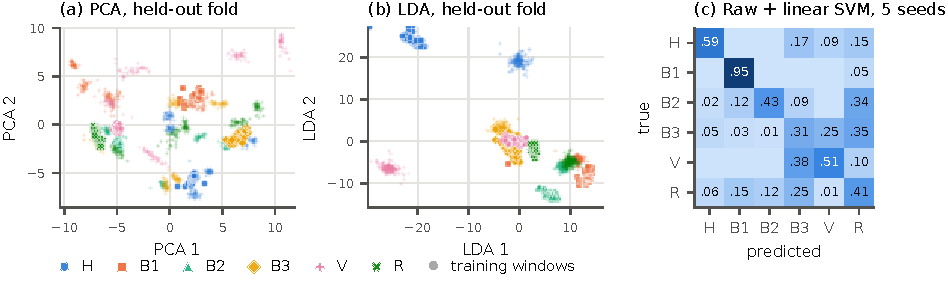
\includegraphics[width=\textwidth]{fig_projection.pdf}
  \end{center}
  \begin{itemize}
    \item Fisher $J$ of LDA-5: about \textbf{490 in-sample}, $15.1 \pm 4.7$ on held-out
          recordings (PCA-5: $10.1 \pm 3.5$).
    \item Held-out recordings land beside the tight training clusters, not in them.
    \item Per class: B1 recall 0.95; H, B3 and V blur together; B2 is often called R.
  \end{itemize}
\end{frame}

\begin{frame}{What survives: lubrication loss \who{Sanika}}
  \begin{columns}[c]
    \begin{column}{0.5\textwidth}
      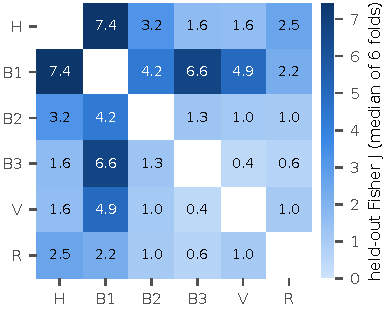
\includegraphics[width=\textwidth]{fig_pair_j.pdf}
    \end{column}
    \begin{column}{0.48\textwidth}
      Held-out $J$ per class pair: 0.4--7.4 (in-sample 600--1{,}600).
      \begin{itemize}
        \item \textbf{B1 separates from every class} ($J$ 2.2--7.4)
        \item against H through impulsiveness: kurtosis ($J = 7.5$), peak-to-peak (4.7),
              impulse factor (4.1)
        \item no defect frequency needed
      \end{itemize}
      B2, B3, V and R form a confusable block. Seed 0.
    \end{column}
  \end{columns}
\end{frame}

\begin{frame}{Hidden: the rotor-bar sidebands \who{Sanika}}
  \begin{center}
    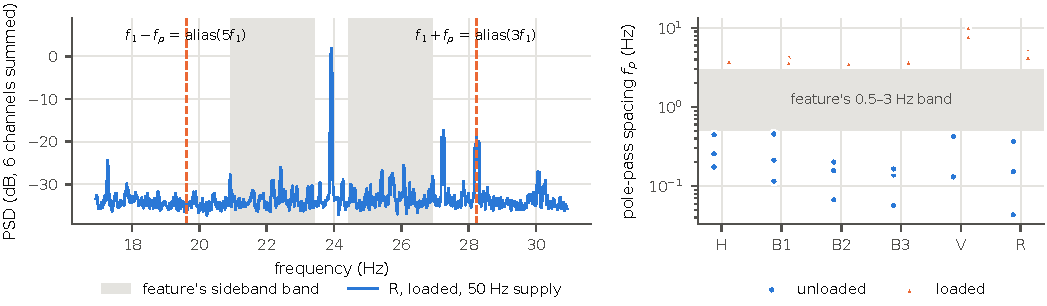
\includegraphics[width=\textwidth]{fig_sidebands.pdf}
  \end{center}
  \begin{itemize}
    \item Measured pole-pass spacing $f_p$: 3.5--10.1\,Hz loaded, $< 0.5$\,Hz unloaded, so
          our 0.5--3\,Hz sideband feature misses it in all 36 recordings.
    \item At 50\,Hz supply, for any slip: $f_1 + f_p = 100 - 3f_1$, the alias of $3f_1$; and
          $f_1 - f_p$ is the alias of $5f_1$. A 100\,Hz sensor cannot tell them apart.
    \item R's one consistent cue is slip under load (median 0.056 vs 0.043--0.047).
  \end{itemize}
\end{frame}

\begin{frame}{Above Nyquist: B3 and V \who{Sanika}}
  \begin{columns}[c]
    \begin{column}{0.5\textwidth}
      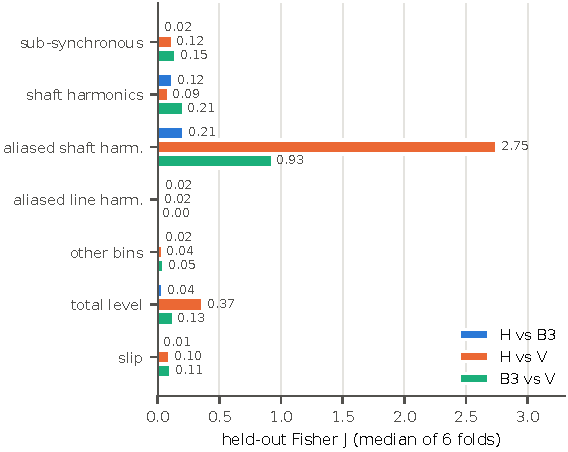
\includegraphics[width=\textwidth]{fig_regions.pdf}
    \end{column}
    \begin{column}{0.48\textwidth}
      \begin{itemize}
        \item Twice line frequency folds to DC at 50\,Hz supply and onto $f_1$ at 40\,Hz.
        \item H vs V: best told apart by energy at \emph{aliased} shaft-harmonic positions
              ($J = 2.75$); V also slips most under load.
        \item H vs B3: no spectral region separates them ($J \le 0.21$); best feature is
              skewness ($J = 1.11$), a waveform asymmetry.
      \end{itemize}
      Seed 0.
    \end{column}
  \end{columns}
\end{frame}

\begin{frame}{Sensor corruption \who{Vaishak}}
  \vspace{-0.6em}
  \begin{center}
    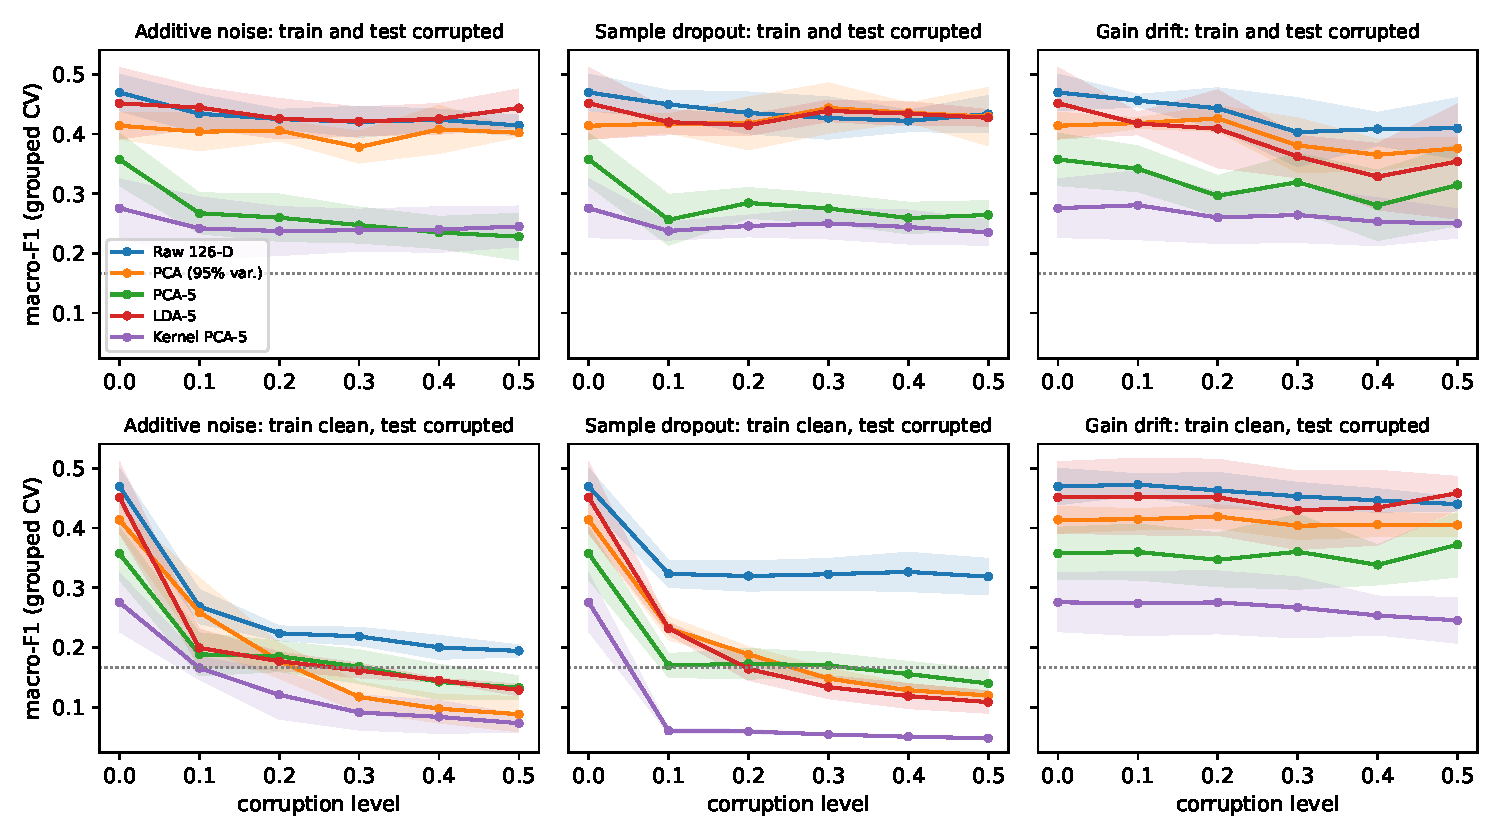
\includegraphics[width=0.74\textwidth]{fig_corruption.pdf}
  \end{center}
  \vspace{-0.6em}
  {\small
  \textbf{Corrupted alike} (top): noise and dropout barely matter; gain drift hurts LDA
  ($0.45 \to 0.35$). \textbf{Trained clean} (bottom): 10\% noise or dropout drops projected
  front-ends to 0.17--0.26; raw features degrade least. Corruption shifts the features, and
  projections fitted on clean data are the most brittle.\par}
\end{frame}

\begin{frame}{Unseen speed and load \who{Vaishak}}
  \begin{center}\resizebox{0.95\textwidth}{!}{\tabfile{tab_ood.tex}}\end{center}
  \vspace{0.4em}
  \begin{itemize}
    \item A new speed is easy ($0.66 \pm 0.02$): 40\,Hz lies between the training speeds.
    \item A new load is the hard shift: it lowers the shaft speed and moves the whole harmonic
          comb. PCA collapses to 0.14--0.15, Kernel PCA to 0.05.
    \item B1 survives the load change; R falls to 0.16 (its slip cue was never seen).
  \end{itemize}
\end{frame}

\begin{frame}{Adapting to the new condition \who{Vaishak}}
  \begin{center}\resizebox{0.9\textwidth}{!}{\tabfile{tab_sa.tex}}\end{center}
  \vspace{0.4em}
  \begin{itemize}
    \item Subspace Alignment (Fernando et al., 2013) uses the target's \emph{unlabelled}
          windows: $M = P_s^\top P_t$.
    \item Adaptation lifts the unseen load from 0.14--0.18 to 0.42--0.60 \dots
    \item \dots\ but per-domain z-scoring does most of it; SA adds $-0.07$ to $+0.09$.
          The shift is mostly location and scale per feature.
  \end{itemize}
\end{frame}

\begin{frame}{Kernel PCA, tuning and DTW do not move the result \who{Sanika}}
  \begin{columns}[c]
    \begin{column}{0.5\textwidth}
      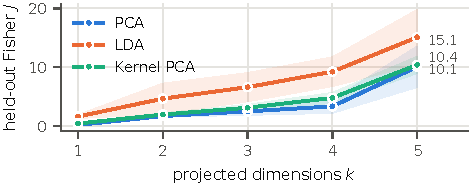
\includegraphics[width=\textwidth]{fig_fisher_k.pdf}
      \vspace{0.3em}
      \resizebox{\textwidth}{!}{\tabfile{tab_dtw.tex}}
    \end{column}
    \begin{column}{0.48\textwidth}
      \begin{itemize}
        \item \textbf{Kernel PCA} keeps PCA's held-out $J$ ($10.4 \pm 1.5$ vs
              $10.1 \pm 3.5$) but classifies worst ($0.28 \pm 0.05$).
        \item \textbf{Nested grouped tuning}: $-0.03$ to $+0.04$ on raw and LDA-5, inside the
              fold-to-fold spread.
        \item \textbf{DTW} on window envelopes: 0.28 vs 0.26 without warping; steady runs
              start at arbitrary phase, so there is nothing to align.
      \end{itemize}
      Tuning and DTW: seed 0.
    \end{column}
  \end{columns}
\end{frame}

\begin{frame}[fragile]{Demo and reproducibility \who{Vaishak \& Sanika}}
  Everything re-runs from the raw data (repository README):
  \vspace{0.3em}
\begin{verbatim}
python scripts/download_data.py        # 36 CSVs + dataset DOI
python scripts/run_baseline.py         # 30-pipeline grid, grouped CV
python scripts/run_corruption.py --corrupt test
python scripts/run_ood.py; python scripts/run_sa.py
python scripts/aggregate_seeds.py      # mean +- std over 5 seeds
python scripts/make_methods_tables.py  # tables and figures
python -m pytest                       # 70 tests
\end{verbatim}
  \begin{itemize}
    \item Every results folder logs seed, parameters, library versions and dataset version.
    \item A fresh clone reproduced every 5-seed table exactly.
    \item Interactive UI (\texttt{ui/}): fault locations, aliasing, feature space, results.
  \end{itemize}
\end{frame}

\begin{frame}{Conclusion \who{Sanika}}
  \begin{itemize}
    \item \textbf{Survives:} lubrication loss, through impulsiveness, even across load.
    \item \textbf{Hidden:} rotor-bar sidebands coincide with aliased shaft harmonics.
    \item \textbf{Above Nyquist:} B3 and V separate only weakly, through asymmetry, slip and
          aliased mechanical harmonics.
    \item Random splits overstate accuracy (1.00 vs 0.47); LDA's in-sample separability is
          recording identity; an unseen load needs per-condition normalisation.
  \end{itemize}
  \vspace{0.5em}
  \textbf{Limits and next steps:} one recording per class and condition, one motor, one
  phone. More recordings, sidebands at the measured $f_p$, training on corrupted data and a
  sensor above 200\,Hz would show which parts of the boundary belong to the faults.
\end{frame}

\end{document}
